\documentclass[12pt]{article}

% --- Paquetes Básicos ---
\usepackage[utf8]{inputenc}
\usepackage[spanish]{babel}
\usepackage[T1]{fontenc}
\usepackage{geometry}
\geometry{a4paper, margin=2.5cm} % Márgenes estándar
\usepackage{setspace}
\setstretch{1.5} % Interlineado 1.5 según norma USS
\usepackage{graphicx}
\usepackage{booktabs}  % Para tablas formato APA
\usepackage{tabularx}

% --- Paquetes Matemáticos y de Símbolos ---
\usepackage{amsmath}   % Esencial para fórmulas avanzadas
\usepackage{amssymb}   % Para símbolos como \leq (menor o igual)
\usepackage{textcomp}  % Para manejar símbolos de texto

% --- Paquetes de Formato y Enlaces ---
\usepackage{hyperref}  % NECESARIO para \texorpdfstring
\hypersetup{
    colorlinks=true,   % True: colorea el texto del link; False: crea un cuadro de color alrededor
    urlcolor=blue,     % Color para los enlaces web externos (formato APA estándar)
    linkcolor=black,   % Color para los enlaces internos (como el índice o notas al pie)
    citecolor=black    % Color para las citas bibliográficas en el texto
}
\usepackage{titlesec}
\usepackage{xcolor}
\usepackage{xurl} % Permite romper las URLs en cualquier carácter para respetar los márgenes

% --- Configuración de Títulos ---
% Definimos niveles para cumplir con tu solicitud de subtítulos y sub-subtítulos
\titleformat{\section}{\normalfont\Large\bfseries}{\thesection}{1em}{}
\titleformat{\subsection}{\normalfont\large\bfseries}{\thesubsection}{1em}{}
\titleformat{\subsubsection}{\normalfont\normalsize\bfseries}{\thesubsubsection}{1em}{}

\begin{document}

% ======================================================
% PORTADA
% ======================================================
\begin{titlepage}
    \centering
    {\bfseries\LARGE Universidad San Sebastián \par}
    \vspace{1cm}
    
\includegraphics[width=0.4\textwidth]{logo_uss.png} \\ % Descomentar y agregar imagen del logo
    \vspace{1cm}
    {\scshape\Large Facultad de Ingeniería \par}
    {\large Carrera de Ingeniería Civil Informática e Ingeniería Civil Industrial \par}
    \vspace{2cm}
    {\bfseries\huge Informe de Álgebra: \par}
    {\Large Análisis Climático y Modelamiento Robótico \par}
    \vspace{3cm}
    
    {\large \textbf{Integrantes:} \par}
    Moises Amundarain \par
    Camila Aravena \par
    Daniela García \par
    María José Santander \par
    Emanuel Ovando \par
    \vfill
    {\large Puerto Montt, Chile \par}
    {\large \today \par} % Fecha automática o puedes poner 18 de mayo de 2026
\end{titlepage}

% ======================================================
% ÍNDICE
% ======================================================
\newpage
\tableofcontents
\newpage

% ======================================================
% INTRODUCCIÓN GENERAL
% ======================================================
\section{Introducción}
El presente informe tiene como objetivo principal analizar y resolver dos problemáticas de ingeniería aplicadas que integran el procesamiento avanzado de datos, el modelamiento geométrico y la abstracción matemática. A través de este desarrollo, se busca vincular los fundamentos teóricos del álgebra lineal y la trigonometría con soluciones computacionales reales y escalables.

En primer lugar, se aborda el estudio analítico de datos climáticos extraídos de la plataforma CAMELS-CL para tres estaciones meteorológicas representativas de las zonas norte, centro y sur de Chile. Mediante la aplicación de lógica de conjuntos y álgebra booleana, se estructuraron las relaciones de cardinalidad para observar empíricamente el comportamiento de variables de temperatura en un quinquenio específico. En segundo lugar, se trabaja en el modelamiento cinemático de un brazo robótico industrial de dos grados de libertad en el plano cartesiano. Utilizando teoremas geométricos oblicuángulos, como la Ley del Coseno y la Ley del Seno, se determinaron los ángulos de articulación necesarios para que el efector final alcance con precisión coordenadas preestablecidas.

Para garantizar la rigurosidad y la reproducibilidad de este proyecto, el equipo de trabajo integró un ecosistema de herramientas tecnológicas de vanguardia. Se utilizó el lenguaje de programación \textbf{Python} junto a la librería \textbf{Pandas} para la limpieza y el análisis masivo de las matrices climáticas, mientras que \textbf{NumPy} y \textbf{Matplotlib} permitieron simular y validar visualmente la estructura espacial del robot. Asimismo, se empleó la \textbf{Inteligencia Artificial (Gemini Pro)} como un asistente crítico en la optimización algorítmica y la auditoría conceptual. Finalmente, la documentación formal del reporte se centralizó mediante el sistema de composición matemática \textbf{LaTeX} en la plataforma TexMaker.

% ======================================================
% CASO 1: ANÁLISIS DE DATOS CLIMÁTICOS (CAMELS-CL)
% ======================================================
\newpage
\section{Caso 1: Análisis de Datos Climáticos}

\subsection{Introducción al Caso}
% Breve contexto sobre el uso de la base de datos CAMELS-CL.

El presente caso de estudio tiene como objetivo central aplicar los fundamentos de la teoría de conjuntos para el análisis de grandes volúmenes de información meteorológica. Para llevar a cabo este propósito, se utiliza la base de datos CAMELS-CL (Catchment Attributes and Meteorology for Large-sample Studies - Chile), una plataforma consolidada que provee registros climáticos históricos y diarios de múltiples estaciones a lo largo del territorio nacional.

El análisis se enfoca en la extracción y clasificación de los registros de temperatura correspondientes a un quinquenio reciente para tres zonas geográficas distintas. Mediante la definición de tres conjuntos matemáticos basados en umbrales térmicos específicos —días con temperaturas máximas superiores a $30^{\circ}\text{C}$, días con mínimas inferiores a $10^{\circ}\text{C}$ y jornadas con un promedio diario entre $18^{\circ}\text{C}$ y $22^{\circ}\text{C}$— se busca calcular sus respectivas cardinalidades y determinar las intersecciones entre ellos. Esta estructuración permite evaluar empíricamente el comportamiento climático, la amplitud térmica de cada región y refutar o confirmar hipótesis de modelos predictivos.

Desde la perspectiva de la Ing. Civil Informática e Ing. Civil Industrial, el procesamiento manual de aproximadamente 1.825 registros por estación resulta un procedimiento ineficiente y vulnerable al error humano. Por consiguiente, la metodología de este estudio integra el desarrollo de algoritmos de automatización mediante el lenguaje de programación Python. La utilización de la librería Pandas\footnote{``Pandas es una librería de Python especializada en el manejo y análisis de estructuras de datos'' (Sánchez Alberca, s.f.).} para la manipulación de los DataFrame\footnote{``Un DataFrame es una estructura de datos que organiza los datos en una tabla bidimensional de filas y columnas, muy parecida a una hoja de cálculo'' (Databricks, s.f.).} garantiza una precisión absoluta en el filtrado de las condiciones lógicas y en el cálculo de las cardinalidades, demostrando cómo las herramientas computacionales optimizan la resolución de problemas en las ciencias aplicadas y el álgebra.

\newpage

\subsection{Registro del procedimiento utilizado}

% Aquí reemplazamos la tabla por subtítulos como solicitaste
\subsubsection{Contar días con temperatura máxima $T > 30^\circ \text{C}$}

\paragraph{Fórmula, función o código utilizado:} % Desarrollo aquí

Se aplicó un filtro booleano\footnote{``Un filtro booleano es una herramienta lógica que utiliza operadores (AND, OR, NOT) para acotar búsquedas, devolviendo solo resultados que cumplen con condiciones de verdadero o falso'' (IBM, s.f.).} sobre la columna de temperatura máxima del DataFrame y luego se sumaron los valores verdaderos para obtener la cardinalidad:
\begin{verbatim}
condicion_A = df['T_max'] > 30
card_A = condicion_A.sum()
\end{verbatim}

\paragraph{Herramienta usada:} % Desarrollo aquí

Para este análisis, usamos dos códigos en Python (librería pandas y os\footnote{``Con la biblioteca \texttt{os}, puedes obtener fácilmente el directorio de trabajo actual. Esto es útil si necesitas saber dónde se encuentra tu script de Python en el sistema de archivos'' (Tech Data Hub, s.f.).}) y archivos .csv\footnote{``Un archivo CSV (por sus siglas en inglés, Comma-Separated Values o Valores Separados por Comas) es un formato de texto plano utilizado para almacenar datos en forma de tabla, donde cada línea representa una fila y los valores de cada columna se separan mediante comas'' (Adobe, s.f.).} para la lectura y guardado de información.

\subsubsection{Contar días con temperatura mínima $T < 10^\circ \text{C}$}

\paragraph{Fórmula, función o código utilizado:} 

Se aplicó un filtro booleano sobre la columna de temperatura mínima del DataFrame y luego se contabilizaron los registros:
\begin{verbatim}
condicion_B = df['T_min'] < 10
card_B = condicion_B.sum()
\end{verbatim}

\paragraph{Herramienta usada:}

Para este análisis, usamos dos códigos en Python (librería pandas y os) y archivos .csv para la lectura y guardado de información.

\subsubsection{Calcular la temperatura promedio diaria}

\paragraph{Fórmula, función o código utilizado:}

Se calculó promediando matemáticamente las columnas de temperatura máxima y mínima para cada día (fila) del DataFrame

\begin{verbatim}
df_unificado['T_mean'] = (df_unificado['T_max'] + df_unificado['T_min']) / 2
\end{verbatim}

\paragraph{Herramienta usada:}

Para este análisis, usamos dos códigos en Python (librería pandas y os) y archivos .csv para la lectura y guardado de información.

\subsubsection{Contar días con $18^\circ \text{C} \leq T_{prom} \leq 22^\circ \text{C}$}

\paragraph{Fórmula, función o código utilizado:}

Se evaluaron dos condiciones simultáneas sobre la columna de temperatura promedio y se sumaron los días que cumplen con el rango inclusivo:
\begin{verbatim}
condicion_C = (df['T_mean'] >= 18) & (df['T_mean'] <= 22)
card_C = condicion_C.sum()
\end{verbatim}

\paragraph{Herramienta usada:}

Para este análisis, usamos dos códigos en Python (librería pandas y os) y archivos .csv para la lectura y guardado de información..

\subsection{Cardinalidades obtenidas y representaciones}
% Aquí se incluirán los resultados de los conjuntos A, B, C y sus intersecciones.

\begin{table}[htbp]
    \centering
    \caption{Cardinalidades obtenidas según zona geográfica}
    \label{tab:cardinalidades}
    \vspace{0.8cm} % Espacio entre el título y la tabla
    
    \begin{tabular}{llccccccc}
        \toprule
        \textbf{Estación} & \textbf{Zona} & \textbf{A} & \textbf{B} & \textbf{C} & $A \cap B$ & $A \cap C$ & $B \cap C$ & $A \cap B \cap C$ \\
        \midrule
        4314002  & Norte  & 0 & 1549 & 0 & 0 & 0 & 0 & 0 \\
        5427003  & Centro & 47  & 1060  & 476 & 0  & 24  & 32  & 0  \\
        10440000 & Sur    & 0 & 1570 & 2 & 0 & 0 & 0 & 0 \\
        \bottomrule
    \end{tabular}
    \vspace{0.5cm}
    
    % Nota al pie de la tabla según formato APA
    \raggedright
    \small \textit{Nota.} Datos procesados a partir de los registros meteorológicos de la base CAMELS-CL correspondientes al último quinquenio disponible.
\end{table}

\subsection{Interpretación de conjuntos e intersecciones}
\subsubsection{Interpretación de $A \cap B$}

Días con temperatura máxima mayor a $30^{\circ}\text{C}$ y temperatura mínima menor a $10^{\circ}\text{C}$, indicando alta amplitud térmica diaria.

\subsubsection{Interpretación de $A \cap C$}

Días con temperatura máxima mayor a $30^{\circ}\text{C}$ y temperatura promedio entre $18^{\circ}\text{C}$ y $22^{\circ}\text{C}$, correspondientes a jornadas cálidas con promedio templado.

\subsubsection{Interpretación de $B \cap C$}

Días con temperatura mínima menor a $10^{\circ}\text{C}$ y temperatura promedio entre $18^{\circ}\text{C}$ y $22^{\circ}\text{C}$, asociada a mañanas frías con temperatura media templada.

\subsubsection{Interpretación de $A \cap B \cap C$}

Días que cumplen simultáneamente las tres condiciones, reflejando alta variabilidad térmica con promedio diario templado.

\subsection{Análisis crítico de datos climáticos}
\subsubsection{Pregunta A: Comparación geográfica de la intersección $A \cap B$}

Al analizar los datos extraídos de las estaciones correspondientes a las zonas Norte, Centro y Sur durante el quinquenio evaluado, se evidencia que la cardinalidad de la intersección $A \cap B$ es exactamente cero (0) en las tres zonas geográficas. Por lo tanto, ninguna presenta una cantidad mayor. 

Climáticamente, esto resulta coherente con las características geográficas del país. Para que un registro pertenezca a la intersección $A \cap B$, debe presentar simultáneamente una temperatura máxima superior a $\texorpdfstring{30^\circ}{\text{C}}$ (Conjunto A) y una mínima inferior a $\texorpdfstring{10^\circ}{\text{C}}$ (Conjunto B) durante el mismo día. Esto exige una amplitud térmica diaria extrema, superior a los $\texorpdfstring{20^{\circ}}{\text{C}}$. 

En Chile, factores geográficos como la alta influencia del Océano Pacífico (que actúa como termorregulador) impiden variaciones diarias tan drásticas en la mayoría de las estaciones, imposibilitando el cumplimiento de ambas condiciones en una sola jornada de 24 horas. Al analizar los datos extraídos de las estaciones correspondientes a las zonas Norte, Centro y Sur durante el quinquenio evaluado, se evidencia que la cardinalidad de la intersección $A \cap B$ es exactamente cero (0) en las tres zonas geográficas. Por lo tanto, ninguna presenta una cantidad mayor. 

\newpage

Climáticamente, esto resulta coherente con las características geográficas del país. Para que un registro pertenezca a la intersección $A \cap B$, debe presentar simultáneamente una temperatura máxima superior a \texorpdfstring{$30^{\circ}\text{C}$}{30 C} (Conjunto A) y una mínima inferior a \texorpdfstring{$10^{\circ}\text{C}$}{10 C} (Conjunto B) durante el mismo día. Esto exige una amplitud térmica diaria extrema, superior a los \texorpdfstring{$20^{\circ}\text{C}$}{20 C}, un fenómeno atípico en la climatología nacional según los registros del Centro de Ciencia del Clima y la Resiliencia [(CR)2] (s.f.).

En Chile, factores geográficos como la alta influencia del Océano Pacífico, que actúa como un potente termorregulador, impiden variaciones diarias tan drásticas en la gran mayoría de las estaciones (Errázuriz et al., 1998). Este efecto moderador imposibilita el cumplimiento de ambas condiciones extremas en una sola jornada de 24 horas, comportamiento que es respaldado por los análisis de eventos térmicos de la Dirección Meteorológica de Chile [DMC] (s.f.).

\subsubsection{Pregunta B: Refutación o confirmación de modelos predictivos en la Zona Sur}

Utilizando la evidencia empírica obtenida del procesamiento computacional para la estación 10440000 (Zona Sur), los datos resultan consistentes con el modelo predictivo, pero son lógicamente insuficientes para confirmarlo de manera absoluta. 

Al analizar los 1583 registros diarios del quinquenio para dicha estación, la cardinalidad del conjunto A (días con $\texorpdfstring{T > 30^\circ}{\text{C}}$) arrojó un valor exacto de cero (0). Sin embargo, la premisa del modelo es una afirmación universal que engloba a todas las estaciones de la zona sur. Metodológicamente, comprobar que la condición se cumple en una sola estación no demuestra que se cumpla en todo el territorio. Para confirmar la premisa, sería imperativo analizar la base de datos de la totalidad de las estaciones del sur; por el contrario, bastaría con encontrar una sola estación que registre un día sobre los $\texorpdfstring{30^\circ}{\text{C}}$ para refutar el modelo por completo.

\newpage

\subsection{Referencias Bibliográficas - Caso 1}
% Espacio para las referencias en formato APA 7ma edición.

\noindent Centro de Ciencia del Clima y la Resiliencia. (s.f.). \textit{Inicio}. Recuperado el 15 de mayo de 2026, de \url{https://www.cr2.cl/} \\

\noindent Dirección Meteorológica de Chile. (s.f.). \textit{Menú temático: Olas}. Recuperado el 15 de mayo de 2026, de \url{https://climatologia.meteochile.gob.cl/application/index/menuTematicoOlas} \\

\noindent Errázuriz, A. M., Cereceda, P., González, J. I., González, M., Gómez, M., y Cunill, P. (1998). \textit{Manual de geografía de Chile}. Editorial Andrés Bello. \url{https://books.google.cl/books?id=oXGaJKGMaMgC} \\

\noindent Databricks. (s.f.). \textit{What are DataFrames?} Recuperado el 15 de mayo de 2026, de \url{https://www.databricks.com/blog/what-are-dataframes} \\

\noindent Adobe. (s.f.). \textit{What is a CSV file?} Recuperado el 15 de mayo de 2026, de \url{https://www.adobe.com/acrobat/resources/document-files/what-is-a-csv-file.html} \\

\noindent IBM. (s.f.). \textit{Campos booleanos}. IBM Documentation. Recuperado el 15 de mayo de 2026, de \url{https://www.ibm.com/docs/es/tap/5.0.0} \\

\noindent Tech Data Hub. (s.f.). \textit{A deep dive into the OS library in Python: Functions, features, and best practices}. Medium. Recuperado el 15 de mayo de 2026, de \url{https://medium.com/tech-data-hub/a-deep-dive-into-the-os-library-in-python-functions-features-and-best-practices-582567bebb06} \\

\noindent Sánchez Alberca, A. (s.f.). \textit{Manual de Pandas}. Aprende con Alf. Recuperado el 16 de mayo de 2026, de \url{https://aprendeconalf.es/docencia/python/manual/pandas/} \\

% ======================================================
% CASO 2: OPTIMIZACIÓN DE BRAZO ROBÓTICO
% ======================================================
\newpage
\section{Caso 2: Optimización de Brazo Robótico}

\subsection{Introducción al Caso}
% Contexto sobre la aplicación de la trigonometría en la cinemática de robots.

El modelamiento matemático y la simulación computacional constituyen pilares fundamentales en el desarrollo de la robótica moderna, la mecatrónica y la automatización industrial. En este ámbito, el análisis cinemático —tanto directo como inverso— es la herramienta que permite determinar la posición espacial del extremo de un mecanismo a partir de los movimientos de sus articulaciones, o bien calcular las configuraciones articulares necesarias para alcanzar un punto objetivo predeterminado.

El presente caso de estudio aborda el análisis geométrico y la optimización cinemática de un brazo robótico plano con dos grados de libertad articulados (configuración antropomórfica o RR\footnote{``La configuración antropomórfica, también conocida como configuración angular, es un tipo de estructura robótica diseñada para imitar la forma y el movimiento del brazo humano'' (SlideShare, s.f.).}). El sistema está compuesto estructuralmente por un primer segmento o brazo de 80~cm ($L_1$) y un segundo segmento o antebrazo de 70~cm ($L_2$). El desafío de ingeniería propuesto consiste en posicionar con precisión absoluta el actuador final del extremo en las coordenadas cartesianas específicas $P(60, 90)$.

Para resolver este problema de cinemática inversa de manera eficiente, se implementa un enfoque analítico algebraico basado en la trigonometría clásica y la resolución de triángulos oblicuángulos. Desde la perspectiva de la Ing. Civil Informática e Ing. Civil Industrial, este modelamiento analítico estructurado representa el paso previo e indispensable para el desarrollo de algoritmos de control de movimiento eficientes en tiempo real. La deducción de soluciones cerradas y exactas optimiza el rendimiento del software, reduciendo drásticamente el costo computacional y el uso de memoria en los sistemas embebidos que gobiernan los servomotores del robot.

\newpage

\subsection{Diseño e implementación del modelo}
% Espacio para la descripción del plano cartesiano y ubicación del punto P(60, 90).


Para determinar analíticamente la configuración espacial requerida por el brazo robótico, es imperativo abstraer la estructura física hacia un modelo geométrico bidimensional en el plano cartesiano. Al fijar la articulación de la base en el origen del sistema de referencia $B(0,0)$ y el efector final en el punto objetivo $P(60,90)$, la articulación intermedia del codo (vértice $C$) se posiciona configurando un triángulo oblicuángulo definido por los nodos $B$, $C$ y $P$.

A continuación, se expone la representación visual teórica del modelo implementado mediante Python y la librería matplotlib\footnote{``Matplotlib es una librería de Python especializada en la creación de gráficos en dos dimensiones'' (Sánchez Alberca, s.f.).}. Este esquema preliminar permite identificar con claridad la disposición espacial de los segmentos ($L_1$ y $L_2$), la recta que define la distancia directa al objetivo ($d$) y las incógnitas angulares constitutivas ($\alpha$ y $\beta$) antes de proceder con el desarrollo analítico exacto:

\begin{figure}[htbp]
    \centering
    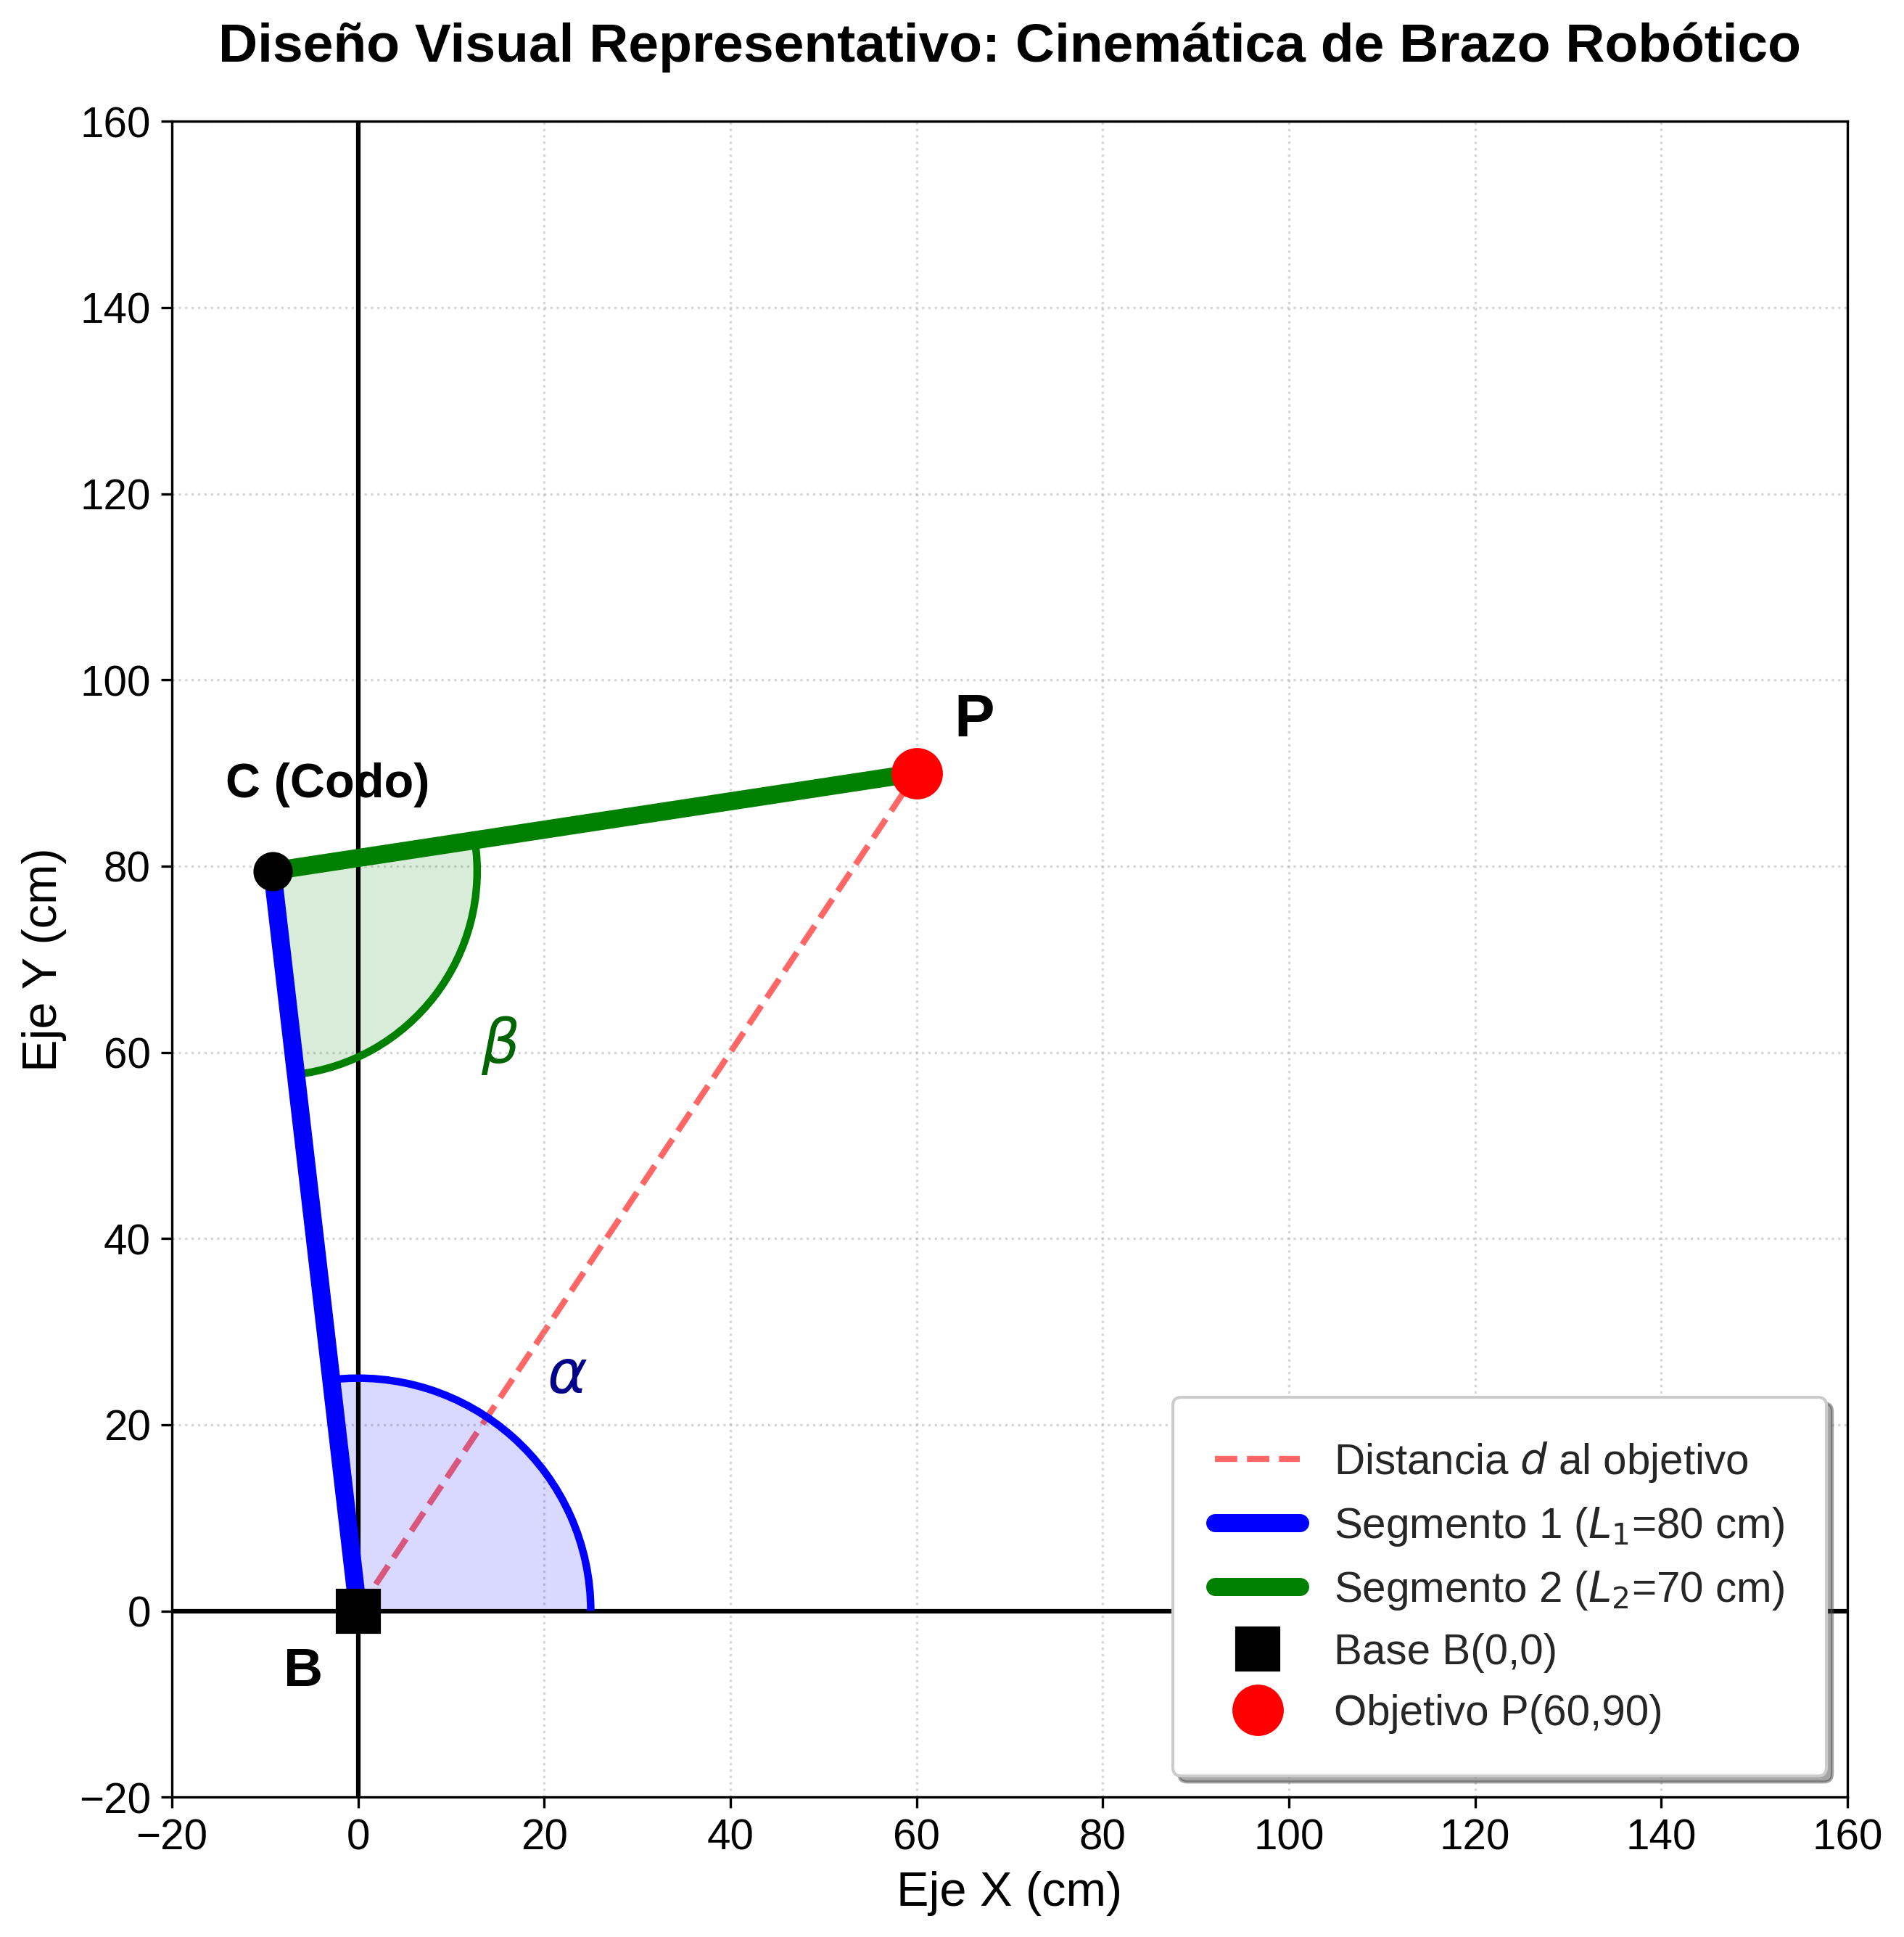
\includegraphics[width=0.7\textwidth]{Diseno_Brazo_Robotico_Teorico.png}
    \caption{Modelamiento geométrico representativo y variables de la cinemática inversa del brazo robótico.}
    \label{fig:brazo_teorico}
\end{figure}

\newpage

\subsection{Análisis cinemático y cálculo de ángulos}
\subsubsection{Cálculo de la distancia euclidiana al punto objetivo}

Para determinar la distancia directa $d$ entre la base del brazo robótico y el efector final, se define la articulación de la base en el origen del sistema de coordenadas $B(x_1, y_1) = (0, 0)$ y el punto objetivo a alcanzar como $P(x_2, y_2) = (60, 90)$. 

Dado que las proyecciones ortogonales del segmento $\overline{BP}$ sobre los ejes cartesianos conforman un triángulo rectángulo con los catetos definidos por las diferencias de las coordenadas, es lícito aplicar el Teorema de Pitágoras mediante la fórmula de la métrica euclidiana. Operando algebraicamente se obtiene:

\begin{align*}
    d^2 &= (x_2 - x_1)^2 + (y_2 - y_1)^2 \\
    \Rightarrow d &= \sqrt{(60 - 0)^2 + (90 - 0)^2} \\
    \Rightarrow d &= \sqrt{(60)^2 + (90)^2} \\
    \Rightarrow d &= \sqrt{3600 + 8100} \\
    \Rightarrow d &= \sqrt{11700} \\
    \therefore d &\approx 108.17 \text{ cm}
\end{align*}

En consecuencia, se demuestra rigurosamente que la distancia euclidiana directa desde el origen hasta el punto objetivo $P$ es de aproximadamente $108.17$ centímetros. Esta magnitud corresponde a la longitud del tercer lado del triángulo oblicuángulo que conformará la cinemática de la estructura.

\subsubsection{Determinación del ángulo interno del codo ($\beta$)}

Basándonos en la abstracción geométrica previa, los segmentos del brazo ($L_1 = 80 \text{ cm}$) y antebrazo ($L_2 = 70 \text{ cm}$) conforman, junto con la distancia euclidiana $d$, un triángulo oblicuángulo. Para determinar el ángulo interno del codo $\beta$, situado en la articulación intermedia y opuesto al lado $d$, se debe aplicar la Ley del Coseno. 

\newpage

Sustituyendo las magnitudes conocidas en la ecuación general, se procede con el siguiente desarrollo algebraico formal:

\begin{align*}
    d^2 = L_1^2 + L_2^2 - 2 \cdot L_1 \cdot L_2 \cdot \cos(\beta) &\implies (\sqrt{11700})^2 = 80^2 + 70^2 - 2(80)(70) \cdot \cos(\beta) \\
    &\implies 11700 = 6400 + 4900 - 11200 \cdot \cos(\beta) \\
    &\implies 11700 = 11300 - 11200 \cdot \cos(\beta) \\
    &\implies 11700 - 11300 = -11200 \cdot \cos(\beta) \\
    &\implies 400 = -11200 \cdot \cos(\beta) \\
    &\implies \cos(\beta) = -\frac{400}{11200} \\
    &\implies \cos(\beta) = -\frac{1}{28} \\
    &\implies \beta = \arccos\left(-\frac{1}{28}\right) \\
    &\implies \beta \approx 92.05^\circ
\end{align*}

Por consiguiente, se demuestra analíticamente que el ángulo interno de flexión requerido en la articulación del codo es de aproximadamente $92.05^\circ$.

\subsubsection{Determinación del ángulo de elevación ($\alpha$)}

Para calcular el ángulo de elevación total $\alpha$ del primer segmento respecto al eje horizontal, el problema se descompone en dos etapas geométricas secuenciales: primero, se determina la orientación angular del vector de posición del punto $P(60,90)$ mediante razones trigonométricas directas; segundo, se calcula el ángulo interno del triángulo oblicuángulo en el vértice de la base utilizando la Ley del Seno.

\newpage

En primer lugar, definiendo $\theta$ como el ángulo agudo que forma el segmento directo $\overline{BP}$ con respecto al eje horizontal positivo, se aplica la función arcotangente sobre las componentes cartesianas del punto objetivo:
\begin{align*}
    \tan(\theta) = \frac{y_2 - y_1}{x_2 - x_1} &\implies \tan(\theta) = \frac{90 - 0}{60 - 0} = 1.5 \\
    &\implies \theta = \arctan(1.5) \\
    &\therefore \theta \approx 56.31^\circ
    \end{align*}

En segundo lugar, se define $\delta$ como el ángulo interno del triángulo oblicuángulo ubicado en el vértice de la base $B$, el cual es adyacente al primer segmento. Sabiendo que el lado opuesto a este ángulo corresponde a la longitud del antebrazo ($L_2 = 70 \text{ cm}$), que la distancia euclidiana es $d \approx 108.17 \text{ cm}$ y que el ángulo del codo opuesto a esta trayectoria es $\beta \approx 92.05^\circ$, se aplica de manera formal la Ley del Seno:
\begin{align*}
    \frac{\sin(\delta)}{L_2} = \frac{\sin(\beta)}{d} &\implies \frac{\sin(\delta)}{70} = \frac{\sin(92.05^\circ)}{108.17} \\
    &\implies \sin(\delta) = \frac{70 \cdot \sin(92.05^\circ)}{108.17} \\
    &\implies \sin(\delta) \approx \frac{70 \cdot 0.99938}{108.17} \\
    &\implies \sin(\delta) \approx 0.6467 \\
    &\implies \delta = \arcsin(0.6467) \\
    &\therefore \delta \approx 40.29^\circ
\end{align*}

Finalmente, por el principio de superposición geométrica en la configuración de codo hacia arriba, el ángulo de elevación total de la base $\alpha$ se obtiene mediante la adición de ambos componentes angulares:
\begin{align*}
    \alpha = \theta + \delta &\implies \alpha = 56.31^\circ + 40.29^\circ \\
    &\therefore \alpha = 96.60^\circ
\end{align*}

De este modo, se demuestra analíticamente que el primer segmento del brazo robótico debe posicionarse con un ángulo de elevación de $96.60^\circ$ respecto a la horizontal para que el actuador final coincida exactamente con las coordenadas del punto objetivo.

\subsection{Modelamiento digital y propiedades geométricas}

Para corroborar la exactitud de los ángulos de configuración obtenidos mediante la resolución analítica ($\alpha \approx 96.60^\circ$ y $\beta \approx 92.05^\circ$), se construyó un modelo computacional paramétrico en el lenguaje de programación Python. Este modelo cumple un doble propósito: renderizar la disposición espacial de los segmentos de longitud fija ($L_1 = 80 \text{ cm}$, $L_2 = 70 \text{ cm}$) respetando la geometría de los ángulos internos, e implementar las ecuaciones de la cinemática directa para calcular la posición resultante del efector final.

A través de las librerías NumPy\footnote{``NumPy es una librería de Python especializada en el cálculo numérico y el análisis de datos, especialmente para un gran volumen de datos'' (Sánchez Alberca, s.f.).} para el cálculo y Matplotlib para el diseño gráfico, el sistema proyecta las coordenadas finales utilizando los ángulos precalculados. Al ejecutar el algoritmo, la consola del sistema entrega el siguiente registro formal de verificación:

\begin{verbatim}
--------------------------------------------------
=== REGISTRO DE VERIFICACIÓN CINEMÁTICA ===
--------------------------------------------------
Objetivo original P : (60, 90)
Ángulo Alpha calculado: 96.60°
Ángulo Beta calculado : 92.05°
Posición Final Alcanzada: (60.00, 90.00)
VALIDACIÓN EXITOSA: Los ángulos posicionan el brazo en P.
--------------------------------------------------
\end{verbatim}

Como se evidencia en la salida computacional y en la gráfica generada (ver Figura \ref{fig:modelo_verificado}), la posición final del eslabón coincide de forma absoluta con las coordenadas del objetivo $P(60,90)$. El sombreado interior confirma empíricamente la disposición del ángulo del codo $\beta$ y la elevación de la base $\alpha$, validando por completo el procedimiento algebraico desarrollado en las secciones anteriores.

\newpage

\begin{figure}[htbp]
    \centering
    % Descomenta la siguiente línea tras subir la imagen a tu proyecto en Overleaf/LaTeX
    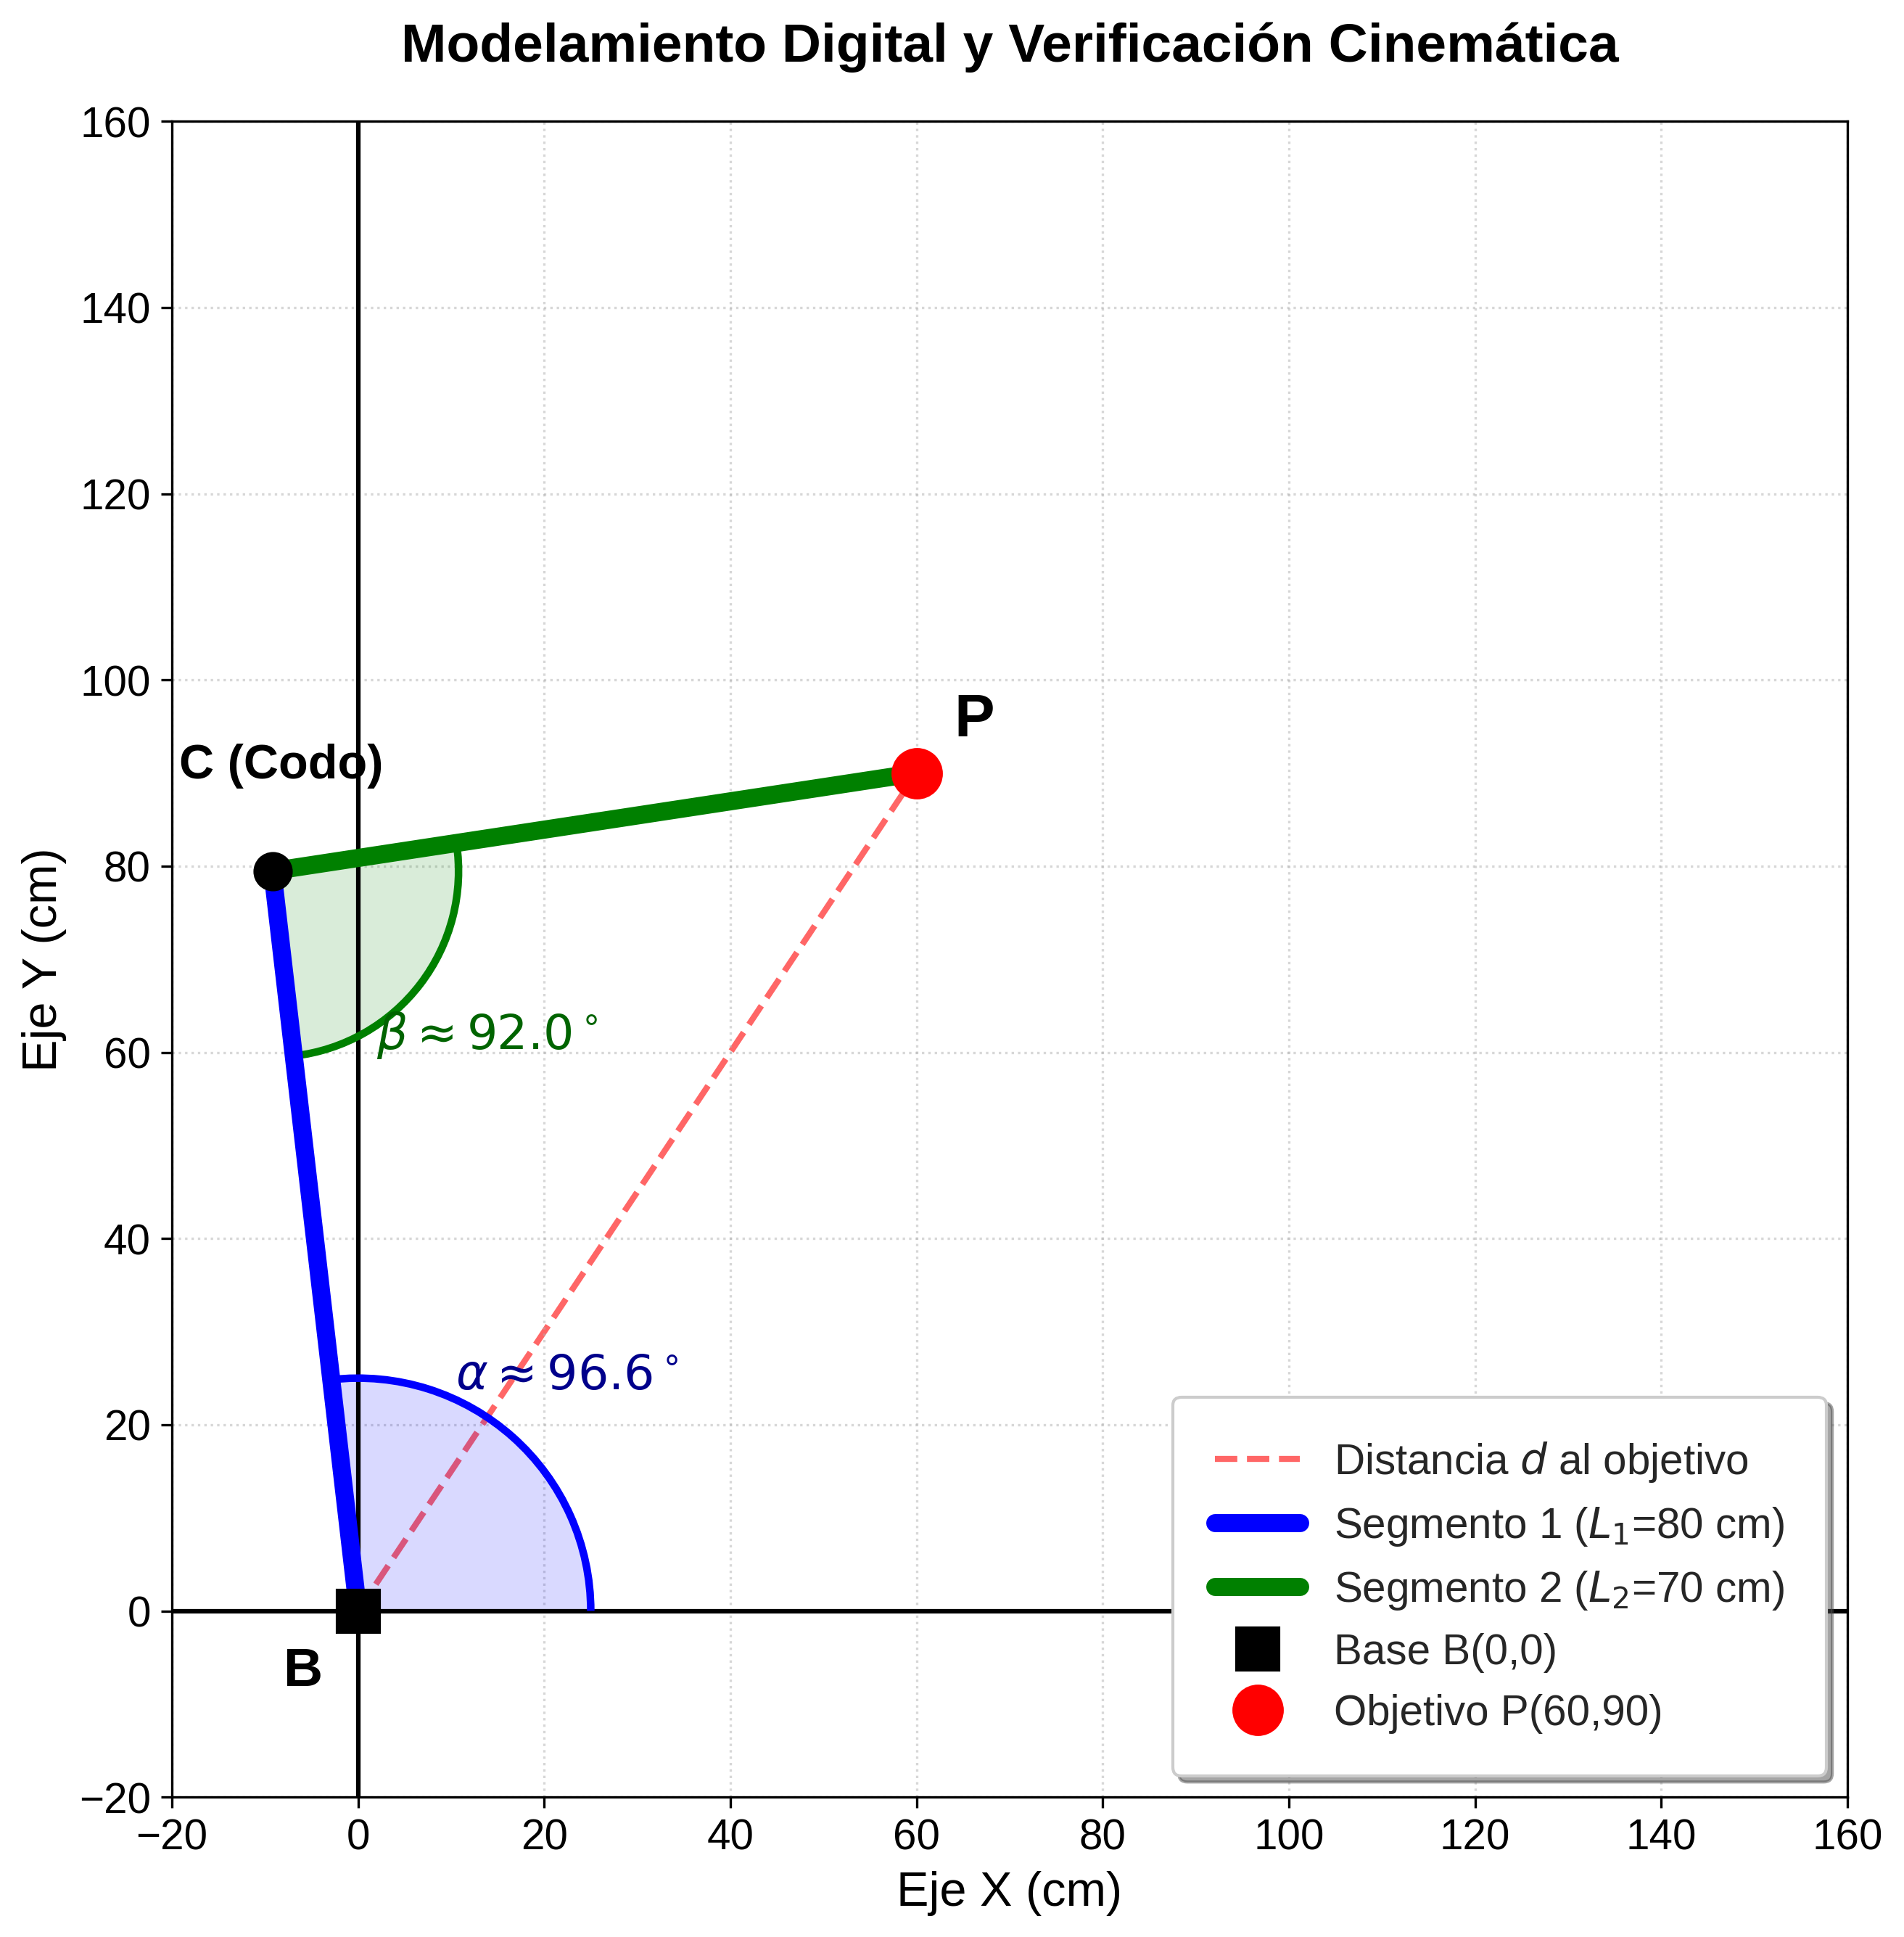
\includegraphics[width=0.85\textwidth]{Modelamiento_Brazo_Verificado_Corregido.png}
    \caption{Representación gráfica del modelamiento digital verificando el alcance del punto objetivo.}
    \label{fig:modelo_verificado}
\end{figure}

\subsection{Configuraciones posibles para el mismo punto}

Sí, efectivamente existen dos configuraciones espaciales posibles para que el brazo robótico alcance el mismo punto objetivo $P(60,90)$, a las cuales se les denomina convencionalmente como configuración de ``codo hacia arriba''\footnote{Codo hacia arriba: ``La articulación del codo se sitúa por encima de la línea recta imaginaria que va desde la base del robot hasta el punto final objetivo'' (Instructables, s.f.).:} y ``codo hacia abajo''\footnote{Codo hacia abajo: ``La articulación del codo queda por debajo de esa línea imaginaria'' (Instructables, s.f.).}. 

\newpage

Desde la perspectiva de la geometría euclidiana, esta dualidad se justifica mediante las propiedades de los triángulos y la simetría axial. Al fijar el punto de la base $B(0,0)$ y el punto objetivo $P(60,90)$, la distancia directa $d$ entre ambos se convierte en un segmento constante. Simultáneamente, las longitudes de los eslabones $L_1$ y $L_2$ son invariables. 


Por el teorema de congruencia LLL (Lado-Lado-Lado), un triángulo cuyos tres lados ($L_1$, $L_2$ y $d$) están definidos tiene una forma y ángulos internos únicos. En consecuencia, el ángulo interno de flexión $\beta$ calculado previamente ($92.05^\circ$) es inalterable. 

No obstante, el triángulo conformado por estos tres segmentos puede construirse en el plano geométrico a ambos lados de la recta que contiene al segmento $\overline{BP}$ (la distancia directa $d$). Esta recta actúa como un eje de simetría. Si reflejamos el vértice del codo $C$ respecto a este eje, obtenemos un segundo vértice $C'$ que preserva exactamente las mismas longitudes $L_1$ y $L_2$ y el mismo ángulo interno $\beta$, pero posicionado en el semiplano opuesto.

Analíticamente, esto significa que el ángulo interno en la base ($\delta \approx 40.29^\circ$) puede sumarse o restarse al ángulo de elevación del vector objetivo ($\theta \approx 56.31^\circ$). 
\begin{itemize}
    \item \textbf{Configuración 1 (Codo arriba):} Calculada en la sección anterior, donde el ángulo de la base es $\alpha_1 = \theta + \delta \approx 96.60^\circ$.
    \item \textbf{Configuración 2 (Codo abajo):} Corresponde a la reflexión simétrica, donde el ángulo de la base sería $\alpha_2 = \theta - \delta \approx 56.31^\circ - 40.29^\circ = 16.02^\circ$.
\end{itemize}

En conclusión, las propiedades de reflexión simétrica de los triángulos demuestran que existen dos posturas articulares válidas para alcanzar el mismo actuador final en el espacio de trabajo bi-dimensional.

\subsection{Verificación del alcance en el punto $(20, 160)$}

Notar que el brazo robótico no posee el alcance físico suficiente para posicionar su efector final en las nuevas coordenadas $P'(20, 160)$. 

\newpage

Para demostrar esta limitación espacial de forma analítica, en primer lugar se procede a calcular la nueva distancia euclidiana $d'$ desde la articulación base $B(0,0)$ hasta el nuevo punto objetivo $P'$:

\begin{align*}
    (d')^2 = (x_2 - x_1)^2 + (y_2 - y_1)^2 &\implies d' = \sqrt{(20 - 0)^2 + (160 - 0)^2} \\
    &\implies d' = \sqrt{20^2 + 160^2} \\
    &\implies d' = \sqrt{400 + 25600} \\
    &\implies d' = \sqrt{26000} \\
    &\therefore d' \approx 161.25 \text{ cm}
\end{align*}

Desde la fundamentación geométrica, el Teorema de la Desigualdad Triangular establece que, para que sea posible construir un polígono cerrado de tres lados (un triángulo), la suma de las longitudes de cualesquiera dos de sus lados debe ser estrictamente mayor que la longitud del tercer lado. Llevado a la cinemática del brazo, para que se logre alcanzar el objetivo, se debe satisfacer la siguiente inecuación:

$$L_1 + L_2 \geq d'$$

Al evaluar esta condición con los parámetros estructurales del modelo ($L_1 = 80 \text{ cm}$ y $L_2 = 70 \text{ cm}$) frente a la nueva distancia calculada:
\begin{align*}
    80 + 70 &\geq 161.25 \\
    150 &\geq 161.25 \quad (\text{Proposición Falsa})
\end{align*}

Dado que $150 \text{ cm} < 161.25 \text{ cm}$, la desigualdad matemática falla. Esto demuestra que la longitud del tercer lado (la distancia al objetivo) supera la suma máxima posible de los dos eslabones. Físicamente, esto significa que el radio máximo del área de trabajo del robot es de $150 \text{ cm}$ (cuando el codo está a $180^\circ$ o totalmente extendido), por lo que el punto $P'(20,160)$ yace fuera de su envolvente de alcance geométrico.


\newpage

\subsection{Referencias Bibliográficas - Caso 2}
% Referencias específicas de cinemática o álgebra lineal.

\noindent SlideShare. (s.f.). \textit{1 Morfología}. Recuperado el 15 de mayo de 2026, de \url{https://es.slideshare.net/slideshow/1-morfologia/54356208} \\

\noindent Sánchez Alberca, A. (s.f.). \textit{Manual de Matplotlib}. Aprende con Alf. Recuperado el 16 de mayo de 2026, de \url{https://aprendeconalf.es/docencia/python/manual/matplotlib/} \\

\noindent Sánchez Alberca, A. (s.f.). \textit{Manual de NumPy}. Aprende con Alf. Recuperado el 16 de mayo de 2026, de \url{https://aprendeconalf.es/docencia/python/manual/numpy/} \\

\noindent Instructables. (s.f.). \textit{Robotic Arm With Gripper}. Recuperado el 16 de mayo de 2026, de \url{https://www.instructables.com/Robotic-Arm-With-Gripper/} \\


\newpage

\section{Registro de herramientas de IA y tecnología}
% Descripción de cómo se usó la IA para el código o validación de cálculos.

\subsection{Registro de herramientas utilizadas}


% Aumentamos el espaciado entre filas para dar espacio para escribir
\renewcommand{\arraystretch}{2}
\noindent
\begin{tabularx}{\textwidth}{@{} l c X @{}}
\toprule
\textbf{Herramienta} & \textbf{¿La utilizó? (Sí/No)} & \textbf{¿En qué parte? (Datos climáticos / Trigonometría / Ambos)} \\
\midrule
Excel & No usamos esta herramienta & En ningura parte\\
GeoGebra & No usamos esta herramienta & En ningura parte\\
Python & Si usamos esta herramienta & Se usó para ambos casos, datos clímaticos y trigonometía \\
Calculadora científica & Si usamos esta herramienta & Se usó para trigonometría \\
IA generativa & Si usamos esta herramienta & Se usó para ambos casos, datos clímaticos y trigonometía\\
Otra: & LaTeX y Word & Se usó para ambos casos, datos clímaticos y trigonometía\\
\bottomrule
\end{tabularx}

\newpage

\subsection{Justificación y reflexión sobre herramientas}

\begin{itemize}
	\item[a)] ¿Para qué utilizó cada herramienta marcada como ``Sí''?
		\begin{itemize}
    \item \textbf{Python:} Se utilizó de manera central en la \textbf{Situación 1} para la extracción, filtrado y procesamiento computacional de los datos climáticos reales provenientes de la base de datos CAMELS-CL. La programación mediante scripts permitió clasificar sin errores los elementos en los conjuntos $A$, $B$ y $C$, y calcular de forma automatizada y exacta todas las cardinalidades e intersecciones, minimizando el error humano frente a grandes volúmenes de datos.
    
    Asimismo, en la \textbf{Situación 2}, se empleó como herramienta de soporte informático para complementar el modelamiento digital, permitiendo validar numéricamente los cálculos trigonométricos obtenidos y verificar las condiciones de la desigualdad triangular para las configuraciones del brazo robótico.
    
    \item \textbf{Calculadora científica:} Fue la herramienta principal para el análisis de la \textbf{Situación 2}. Se requirió para ejecutar los cálculos aritméticos al aplicar la Ley del Coseno y las razones trigonométricas (o Ley del Seno), permitiendo determinar los valores exactos de los ángulos $\alpha$ y $\beta$ para posicionar el extremo del brazo robótico en el punto $P(60, 90)$.
    
    \item \textbf{IA generativa:} Actuó como una herramienta de apoyo y consulta durante el desarrollo de la prueba. Se empleó principalmente para la comprensión conceptual de ciertos bloqueos, apoyo en la generación o depuración de código para el análisis de datos, y como asistencia para estructurar el formato de las justificaciones y conclusiones requeridas en el análisis crítico.
    
    \item \textbf{LaTeX y Word:} Se utilizaron para la redacción, consolidación y formato final del informe. Permitieron cumplir con la estructura exigida (introducción, desarrollo analítico y conclusión), asegurando que el desarrollo de las ecuaciones algebraicas y trigonométricas se presentara con el máximo rigor académico, limpieza y legibilidad.
    
    \newpage
\end{itemize}
	\item[b)] ¿Por qué las herramientas seleccionadas fueron adecuadas para las tareas realizadas?
		
		Las herramientas seleccionadas resultaron adecuadas porque cada una cubrió una necesidad técnica específica exigida por las situaciones del problema, optimizando el tiempo y minimizando el error humano.

\begin{itemize}
    \item \textbf{Eficiencia frente a datos reales (Python):} Trabajar con la base de datos climáticos CAMELS-CL en la \textbf{Situación 1} implicaba procesar grandes volúmenes de información. Python automatizó el filtrado, la clasificación de los conjuntos $A$, $B$ y $C$, y el cálculo de sus cardinalidades, lo que de forma manual sería ineficiente y propenso a errores. Asimismo, permitió validar numéricamente las restricciones en la \textbf{Situación 2}.
    
    \item \textbf{Precisión en el modelamiento (Calculadora científica):} Para la \textbf{Situación 2}, la aplicación de la Ley del Coseno y del Seno requería calcular funciones trigonométricas inversas. La calculadora fue fundamental para obtener los valores exactos de los ángulos $\alpha$ y $\beta$, asegurando que el brazo alcanzara con precisión el punto $P(60, 90)$.
    
    \item \textbf{Soporte y optimización del tiempo (IA generativa):} Resultó adecuada como asistente metodológico. Permitió resolver bloqueos conceptuales, depurar errores sintácticos en los scripts de Python y ayudó a estructurar la redacción de los argumentos reflexivos.
    
    \item \textbf{Rigor académico y claridad visual (LaTeX y Word):} Garantizaron que las justificaciones, el análisis crítico y el desarrollo algebraico y trigonométrico se presentaran de forma profesional, ordenada y cumpliendo con la estructura exigida en la rúbrica.
\end{itemize}
 \newpage
	\item[c)] ¿Qué herramienta le resultó más útil para el análisis de datos climáticos y por qué?
	
	Para el análisis de la base de datos climática CAMELS-CL (Caso 1), la herramienta tecnológica más útil y determinante fue el lenguaje de programación \textbf{Python}, específicamente a través de su librería \textbf{Pandas}.

La justificación principal radica en el volumen y la naturaleza estructurada de la información. Al tratar con registros meteorológicos diarios (temperaturas máximas y mínimas) documentados a lo largo de un quinquenio completo, el procesamiento manual o la utilización de hojas de cálculo tradicionales resultaba ineficiente y estadísticamente propenso a errores humanos. 

Mediante el uso de Pandas, fue posible abstraer la manipulación de grandes volúmenes de información a través de DataFrames, lo que permitió automatizar procesos matemáticos y lógicos críticos, tales como:
\begin{itemize}
    \item La limpieza y depuración automatizada de valores nulos o registros corruptos mediante el comando \texttt{dropna()}.
    \item El cálculo aritmético masivo de la temperatura promedio diaria (\texttt{T\_mean}) cruzando matrices de datos en fracciones de segundo.
    \item La aplicación de lógica booleana matricial para aislar los conjuntos climáticos ($A$, $B$ y $C$) y calcular las cardinalidades de sus intersecciones exactas (ej. $A \cap B \cap C$) mediante operadores lógicos.
\end{itemize}

Desde la perspectiva de la Ing. Civil Informática e Ing. Civil Industrial, estructurar esta solución analítica mediante scripts automatizados no solo garantizó la precisión algorítmica requerida para la resolución del problema, sino que también otorgó escalabilidad al proyecto. Gracias a esta herramienta, el modelo desarrollado es universal, permitiendo procesar instantáneamente la información de cualquier otra estación meteorológica de Chile sin necesidad de reescribir la lógica de fondo.
\newpage
	\item[d)] ¿Qué herramienta le resultó más útil para el modelamiento geométrico/trigonométrico y por qué?
	
	Para el modelamiento geométrico y trigonométrico del brazo robótico de dos grados de libertad (Caso 2), la herramienta más útil y significativa fue la combinación de \textbf{Python} junto con las librerías científicas \textbf{NumPy} y \textbf{Matplotlib}.

Si bien el análisis abstracto inicial se fundamentó en teoremas geométricos puros (como la Ley del Coseno, el Teorema de Pitágoras y la Desigualdad Triangular), la programación en Python permitió trasladar esas ecuaciones analíticas estáticas a un entorno dinámico y visual. Las razones principales de su utilidad se desglosan a continuación:

\begin{itemize}
    \item \textbf{Precisión y cálculo trigonométrico robusto:} La utilización de NumPy fue fundamental para gestionar funciones trigonométricas inversas (arccos y arctan) utilizando arreglos vectoriales. Esto evitó los errores de redondeo manual y permitió operar con alta precisión decimal los ángulos de elevación ($\alpha$) y del codo ($\beta$).
    \item \textbf{Validación inmediata del modelo:} A diferencia de herramientas gráficas estáticas, programar las ecuaciones de cinemática directa en Python sirvió como un entorno de pruebas definitivo. Al ingresar los ángulos calculados manualmente, el script calculó la posición final del efector, ratificando algebraicamente que coincidía de forma exacta con las coordenadas del punto objetivo $P(60, 90)$.
    \item \textbf{Representación geométrica fidedigna:} A través de Matplotlib, se logró vectorizar el comportamiento físico del robot, graficando los eslabones como segmentos de longitud fija ($L_1 = 80 \text{ cm}$ y $L_2 = 70 \text{ cm}$), delimitando los vértices principales de la estructura y sombreando los arcos internos de los ángulos mediante el uso avanzado de parches geométricos (\textit{Wedges}).
\end{itemize}

En el marco de la informática, esta metodología demostró la importancia de la simulación computacional, probando que el código no solo es una herramienta de cálculo, sino un medio para interpretar, verificar y visibilizar propiedades geométricas abstractas en una aplicación real de la robótica.

\newpage
	\item[e)] ¿Existió alguna herramienta que intentó utilizar pero no resultó adecuada? Explique.
	
No hubo una herramienta que quisiéramos utilizar y no haya funcionado, ya que, como equipo, logramos identificar desde el primer momento las herramientas que íbamos a necesitar y supimos que estas iban a funcionar.
	
\end{itemize}

\subsection{Uso de Inteligencia Artificial}

\begin{itemize}
	\item[a)] ¿Qué plataforma(s) utilizó?
	
	Para el desarrollo coordinado, estructuración y auditoría de los Casos 1 y 2, se utilizó de manera exclusiva la plataforma de Inteligencia Artificial \textbf{Gemini} (en su versión avanzada con el modelo \textit{Gemini Pro}), operando como un asistente de ingeniería en tiempo real.
	
	\item[b)] ¿Qué tipo de ayuda solicitó?
	
	Se solicitaron tres tipos de asistencia complementaria a lo largo del proyecto:
    \begin{itemize}
        \item \textbf{Auditoría y revisión de cálculos analíticos:} Validación y corrección de la sintaxis matemática de los desarrollos manuales generados por el equipo (Teorema de Pitágoras, Ley del Coseno y Ley del Seno).
        \item \textbf{Optimización y refactorización de código:} Depuración de scripts en Python para la automatización de la lectura de matrices climáticas en Pandas y corrección de la lógica de renderizado geométrico de parches de ángulos en Matplotlib.
        \item \textbf{Maquetación académica:} Transposición de los textos explicativos, inecuaciones y tablas de la rúbrica al lenguaje de tipografía matemática \textbf{LaTeX} bajo estándares formales.
    \end{itemize}
    
	\item[c)] Indique un resultado útil generado por IA.
	
	El resultado más útil y de mayor impacto técnico fue la \textbf{resolución del algoritmo de lógica vectorial para el sombreado del codo} en el modelo digital de Python. La IA estructuró de manera exacta el cálculo de los ángulos absolutos desde la articulación intermedia utilizando la función \texttt{arctan}, proveyendo las condiciones lógicas necesarias para obligar a la librería Matplotlib a trazar el arco (\textit{Wedge}) estrictamente en el trayecto interno del triángulo del brazo, logrando una simulación física e informática fidedigna.
	
	\item[d)] Indique un error o limitación detectada en la respuesta de IA.
	
	Se detectó un \textbf{error de alucinación e indexación de datos} en la primera propuesta de generación gráfica del brazo robótico. El modelo de IA configuró de manera errónea el orden de los vectores directores de la articulación, lo que provocó que el arco sombreado del codo ($\beta$) se renderizara invertido hacia el exterior de la estructura (ángulo reflejo de más de $260^\circ$) en lugar de acotarse al interior del triángulo oblicuángulo, además de posicionar la etiqueta del texto numérico fuera de los márgenes visibles del gráfico.
	
	\item[e)] Indique una verificación manual que debió realizar.
	
	Se debió realizar una \textbf{auditoría conceptual y de vocabulario geométrico} sobre las explicaciones matemáticas generadas. El equipo tuvo que intervenir manualmente las primeras descripciones de la IA y de los borradores grupales para eliminar por completo términos como ``catetos'' e ``hipotenusa'' en el análisis de la Ley del Coseno y del Seno, reemplazándolos de forma rigurosa por ``segmentos'' y ``longitudes de eslabones'', dado que dichos conceptos trigonométricos pertenecen exclusivamente a triángulos rectángulos y no a la naturaleza oblicuáugula de la cinemática del robot. Asimismo, se auditó manualmente que el resultado numérico del código de cinemática directa coincidiera con la distancia real obtenida analíticamente.

\end{itemize}


% ======================================================
% CONCLUSIÓN Y CIERRE
% ======================================================
\newpage
\section{Conclusión General}
% Reflexión final sobre el uso de herramientas tecnológicas en la resolución de problemas de ingeniería.

El desarrollo integral de este informe ha permitido consolidar una visión práctica, interdisciplinaria y de alto nivel sobre cómo las herramientas computacionales avanzadas transforman la abstracción matemática en soluciones tangibles para problemas reales de ingeniería. A través de la resolución de los dos casos de estudio planteados, se han validado conceptos fundamentales del álgebra, la lógica y la trigonometría, demostrando su relevancia en el análisis de datos masivos y en la automatización industrial.

En el primer caso, centrado en el análisis de los datos climáticos de la base de datos CAMELS-CL, la implementación del álgebra de conjuntos y la lógica booleana mediante el lenguaje de programación Python resultó indispensable. La manipulación analítica tradicional de registros meteorológicos diarios a lo largo de un quinquenio habría sido ineficiente y propensa a imprecisiones estadísticas. La automatización mediante librerías científicas no solo garantizó la obtención exacta de las cardinalidades e intersecciones climáticas en las zonas norte, centro y sur de Chile, sino que dotó al proyecto de escalabilidad, demostrando el valor de estructurar algoritmos genéricos y universales capaces de procesar de forma inmediata cualquier estación del país.

Por otro lado, el segundo caso abordó el modelamiento cinemático de un manipulador robótico de dos grados de libertad en el plano cartesiano. Este desafío evidenció el vínculo directo entre la geometría analítica pura —sustentada en el Teorema de Pitágoras, la Ley del Coseno y la Ley del Seno— y la simulación digital. La transición desde hojas de cálculo estáticas tradicionales hacia un entorno de desarrollo paramétrico en Python (con NumPy y Matplotlib) fue crítica. Esto no solo sirvió como un método de verificación empírica para corroborar que los ángulos calculados manualmente posicionaban el efector exactamente en las coordenadas objetivo $P(60, 90)$, sino que además permitió superar restricciones técnicas complejas de renderizado vectorial y lógica de cuadrantes para representar fielmente la anatomía espacial del robot.

\newpage

Finalmente, el proceso de desarrollo grupal reafirmó la importancia de adoptar un enfoque crítico y reflexivo frente al uso de herramientas de Inteligencia Artificial. Lejos de actuar como un sustituto del criterio de ingeniería, el uso de asistentes avanzados requirió de una constante auditoría conceptual por parte del equipo, tanto en la corrección de alucinaciones gráficas de inversión de ángulos como en la depuración del vocabulario riguroso empleado en las justificaciones matemáticas. En definitiva, este proyecto demuestra que el perfil del Ingeniero/a Civil Informático/a e Ingeniero/a Civil Industrial moderno no se limita a la escritura de código o a la resolución algebraica aislada, sino a la capacidad de integrar de manera armónica las matemáticas, la programación y el control de versiones bajo estándares académicos de excelencia tipográfica (LaTeX), sentando las bases para afrontar con éxito desafíos técnicos de mayor complejidad.

\end{document}